		Once all prior processes have been completed, the results of classification are output in two forms, as a GUI and on the system console. The GUI output is illustrated in the figure below:
		
		\begin{figure}[H]
			\centering
			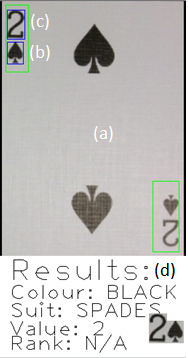
\includegraphics[width=0.4\textwidth]{chris/image33}
			\caption{Card classification GUI output showing card isolated (a), isolated suit symbol (b), isolated rank symbol (c) and textual results output (d).}
		\end{figure}

		For each detected card in the input image, the classified suit colour, suit symbol, value (0 for picture cards) and the rank detected (N/A for number cards).
		
		In this method of output it is easy to determine which elements of classification have succeeded or why they have failed when they do. For example, the isolated suit and rank symbol image matrices are reproduced at the bottom of the window, and therefore in the event of a problem in classification the intermediary isolations can be checked for errors. 
		
		The second form of output is shown in the form of a natural language result in the system console. A string is concatenated using all the fields stored in the Card structure once classification is complete to form a single plain-English sentence. The code segment below illustrates how this is done:

		\begin{lstlisting}

//Nice CMD summary
cout << endl << "============== Detected Cards ==============" << endl << endl;

for(size_t i = 0; i < cards.size(); i++)
{
    cout << "Card " << (i + 1) << ": The ";

    if(cards[i].is_picture_card)
    {
        switch(cards[i].detected_rank)
        {
        case Card::RANK_JACK:
            cout << "Jack";
            break;
        case Card::RANK_QUEEN:
            cout << "Queen";
            break;
        case Card::RANK_KING:
            cout << "King";
            break;
        case Card::RANK_ACE:
            cout << "Ace";
            break;
        default:
            cout << "Something";
            break;
        }
    }
    else
    {
        cout << cards[i].detected_value;
    }

    cout << " of ";

    switch(cards[i].detected_suit)
    {
    case Card::CLUBS:
        cout << "Clubs";
        break;
    case Card::DIAMONDS:
        cout << "Diamonds";
        break;
    case Card::HEARTS:
        cout << "Hearts";
        break;
    case Card::SPADES:
        cout << "Spades";
        break;
    default:
        cout << "Something";
        break;
    }

    cout << endl;
}

cout << endl << "============================================" << endl << endl;
		\end{lstlisting}

		This is repeated for each card in the cascade, and is shown below for an example cascade of classified cards:

		\begin{figure}[H]
			\centering
			\begin{subfigure}[b]{\textwidth}
				\centering
				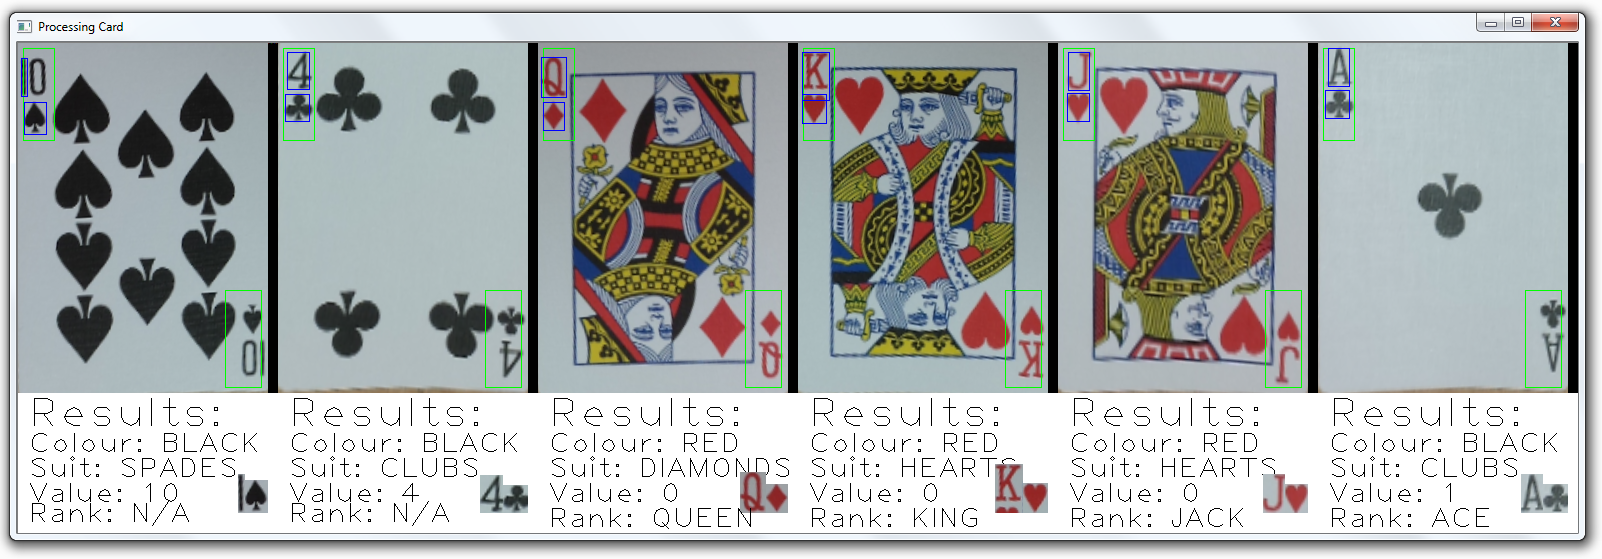
\includegraphics[width=\textwidth]{chris/image34}
				\caption{}
			\end{subfigure}
		\end{figure}
		\begin{figure}[H]
			\ContinuedFloat
			\centering
			\begin{subfigure}[b]{\textwidth}
				\centering
				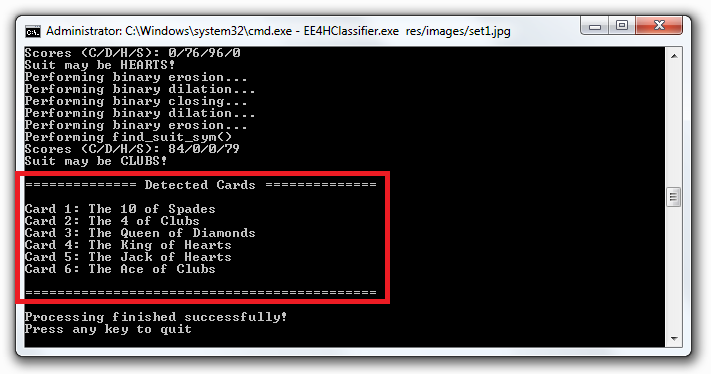
\includegraphics[width=\textwidth]{chris/image35}
				\caption{}
			\end{subfigure}
			\caption{Example correct classification cascade of six cards showing GUI (a) and console output (b) formats.}
		\end{figure}

		A criterion for improvement for future expansion or interoperability of the software with other systems could be a CSV (comma separated values) output or network connectivity, both of which are not too difficult to implement.